\makeatletter
\def\input@path{{../}}
\makeatother

\documentclass[/main.tex]{subfiles}
\graphicspath{{./pics/}{appSens/pics/}}
\begin{document}

\onlyinsubfile{\appendix}
\chapter{Sensitivity and Discovery Potential}
\label{app:sens}

When performing rare event searches in the presence of backgrounds, it is often useful to select regions of interest and data cleaning cuts that optimize the experimental sensitivity.
Median n-$\sigma$ count sensitivity, $\hat{S}(\overline{B}, n_\sigma)$ is defined as the median upper limit of an n-$\sigma$ confidence interval on the number of observed signal counts, assuming the presence of no signal and backgrounds sampled from a distribution based on measured background level $\overline{B}$.
A similar quantity, n-$\sigma$ discovery sensitivity, is defined as the true strength of a signal that would produce a discovery with significance n-$\sigma$ 50\% of the time.
Unlike median sensitivity, discovery sensitivity accounts for the distribution in the number of counts that would be seen based on the true rate.
For this reason, discovery sensitivity is a slightly more useful quantity when projecting or optimizing an experiment's sensitivity, even though median (or mean) sensitivity is the quantity that is usually reported.
For the purpose of this appendix, we will focus on discovery sensitivity.

The sensitivity of the experiment to the total rate of the process being searched for is
\begin{equation}
  \hat{\Gamma}(\overline{B}, \epsilon, n_\sigma)\propto\frac{\hat{S}(\overline{B}, n_\sigma)}{\epsilon}
\end{equation}
where $\epsilon$ is the total detection efficiency of the signal being sought.
Optimizing event selection for a search requires balancing the tradeoff between reducing backgrounds, which will decrease $\hat{S}(\overline{B})$, and improving signal detection efficiency.

When optimizing a search, it is useful to use certain approximations when calculating sensitivity.
In the high background limit, a common approximation is to assume the backgrounds measured will have a gaussian distribution with standard deviation of $\sqrt{\overline{B}}$.
In this case, the discovery (and median) sensitivity will be
\begin{equation}
  \hat{S}(\overline{B}, n_\sigma)=n_\sigma * \sqrt{\overline{B}}
\end{equation}

This approximation fails, however, in the low background limit, where a better approximation is that the background will instead be sampled from a Poisson distribution with mean counts $\overline{B}$.
Because the Poisson distribution is a PDF over a discrete variable, the resultent sensitivity will have step-like properties and must be solved for using a toy Monte Carlo, properties that are not ideal for performing sensitivity optimizations.
For this reason, when computing the sensitivity we instead use the analytic continuation of the CDF of the poisson distribution, which is the lower incomplete gamma function
\begin{equation}
  \gamma(s, x)=\frac{1}{\Gamma(s)}\int_0^x t^{s-1} \mathrm{e}^{-t} \mathrm{d}t
\end{equation}
In this case, we can find the sensitivity, by first numerically solving for the number of counts required for an n-sigma discovery, $\hat{N}$, with expected backgrounds $\overline{B}$, where
\begin{equation}
  \gamma(\hat{N}+1, \overline{B}) = \mathrm{erfc}(\frac{n_\sigma}{\sqrt{2}})
\end{equation}
To get the median sensitivity, we then numerically solve
\begin{equation}
  \gamma(\hat{N}+1, \overline{B} + \hat{S}) = 0.5
\end{equation}
We define the function found by solving these equations to be the discovery potential\cite{2013CUORE},
\begin{equation}
  \hat{S}(\overline{B}, n_\sigma) = \mathrm{DP}(\overline{B}, n_\sigma)
\end{equation}
For the purposes of this dissertation, we always use the 3-sigma discovery potential
\begin{equation}
  \mathrm{DP}(\overline{B}) = \mathrm{DP}(\overline{B}, 3)
\end{equation}
Figure~\ref{fig:DPvSens} shows a comparison of the gaussian approximation for sensitivity to the discovery potential.
This function is implemented in \texttt{GATPeakShapeUtils.hh} as \linebreak\texttt{GATPeakShapeFunction::DiscoveryLimit}.

\begin{figure}[h]
  \centering
  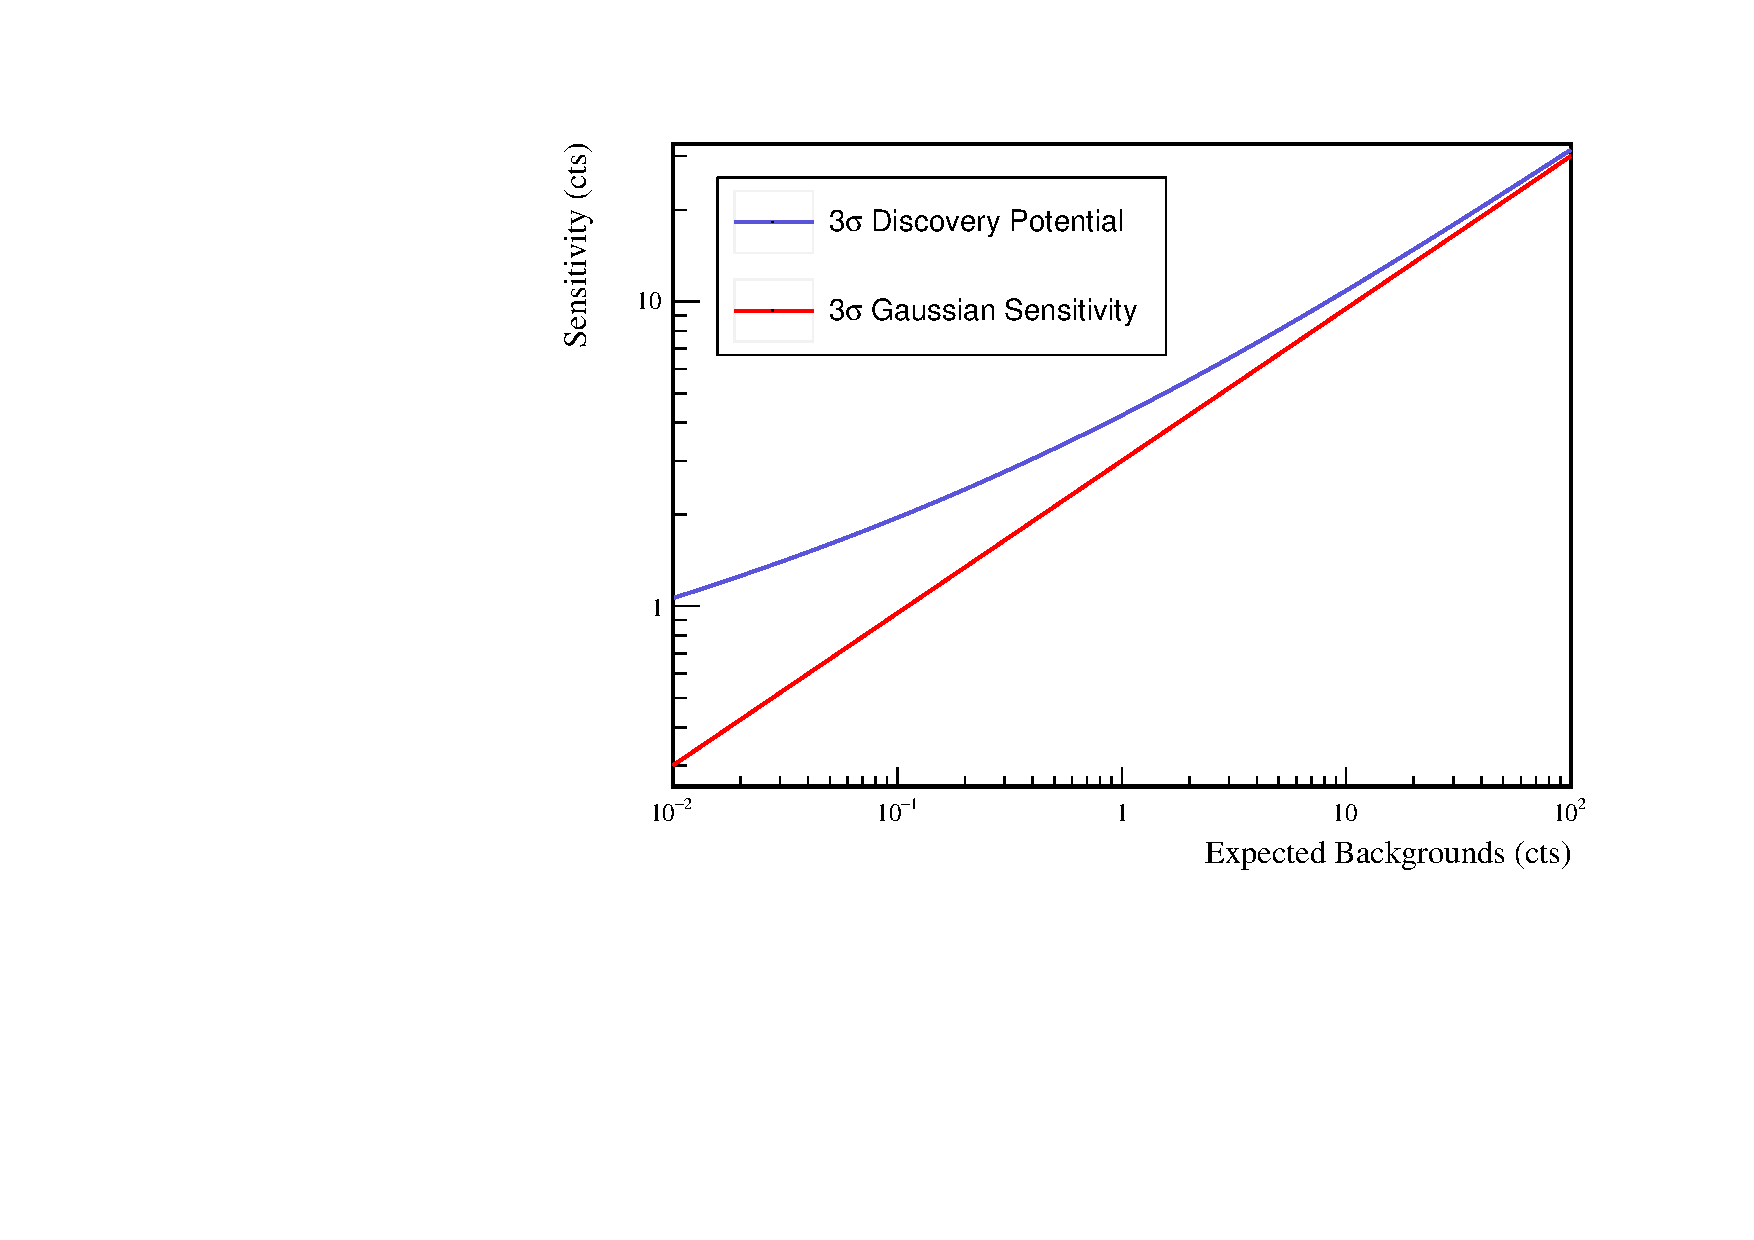
\includegraphics[width=0.8\textwidth]{DPvSens}
  \caption[Comparison between sensitivity in Gaussian background approximation and Discovery Potential] {\label{fig:DPvSens}
    A comparison of the Gaussian approximation for sensitivity and the discovery potential as a function of expected background level. Note that in the high background limit, both formulations for sensitivity converge, as expected.
    }
\end{figure}
Next, we want to figure out how we will use these quantities to optimize our data selection.
To determine whether it is worth adding a cut or modifying a cut, consider the efficiency and expected background counts before and after applying the cut ($\epsilon_i$, $\overline{B}_i$ and $\epsilon_f$, $\overline{B}_f$, respectively).
A cut represents an improvement if
\begin{equation}
  \frac{\hat{S}(\overline{B}_f)}{\epsilon_f} <\frac{\hat{S}(\overline{B}_i)}{\epsilon_i}
\end{equation}
Rearranging this, we get
\begin{equation}
  \frac{\Delta \hat{S}(\overline{B})}{\hat{S}(\overline{B_i})} < \frac{\Delta\epsilon}{\epsilon_i}
\end{equation}
If we assume that a small number of events are cut, we can Taylor expand:
\begin{equation} \label{eq:cutcriterion}
  \frac{\partial\hat{S}}{\partial\overline{B}} \frac{\Delta\overline{B}}{\hat{S}(\overline{B})} < \frac{\Delta\epsilon}{\epsilon}
\end{equation}
\begin{equation}
  \frac{\partial\log(\hat{S})}{\partial\log(\overline{B})} > \frac{\mathrm{False~Positive~Rate}}{\mathrm{True~Positive~Rate}}
\end{equation}
Looking at figure~\ref{fig:DPvSens}, we see that in the high background limit, using the Gaussian sensitivity approximation we will draw the same conclusion about whether or not a cut is worth applying regardless of the absolute background level.
A cut is worth applying as long as the true positive rate of the cut is twice the true negative rate.
On the other hand, in the low background limit, this is not the case; instead, as we approach zero background, we will be less aggressive in cutting events.
For this reason, experiments approaching the background free limit will use wider regions of interest in peak searches.

\onlyinsubfile{
  \bibliographystyle{plain}
  \bibliography{../main}
}

\end{document}